\documentclass[conference]{IEEEtran}
\IEEEoverridecommandlockouts
\usepackage{cite}
\usepackage{amsmath,amssymb,amsfonts}
\usepackage{algorithmic}
\usepackage{graphicx}
\usepackage{textcomp}
\usepackage{xcolor}
\usepackage{tikz}
\usetikzlibrary{arrows.meta, positioning, fit, backgrounds}
\def\BibTeX{{\rm B\kern-.05em{\sc i\kern-.025em b}\kern-.08em
    T\kern-.1667em\lower.7ex\hbox{E}\kern-.125emX}}
\begin{document}

\title{Obstacle Recognition: Real-Time Event-Based Optical Avoidance on Edge Devices\\

}

\author{\IEEEauthorblockN{1\textsuperscript{st} Paweł Jerzyna}
\IEEEauthorblockA{\textit{Faculty of Electrical Engineering, Automatics, Computer Science and Biomedical Engineering} \\
\textit{AGH University of Krakow}\\
Kraków, Poland \\
jerzyna@student.agh.edu.pl}
\and
\IEEEauthorblockN{2\textsuperscript{nd} Piotr Grzyb}
\IEEEauthorblockA{\textit{Faculty of Electrical Engineering, Automatics, Computer Science and Biomedical Engineering} \\
\textit{AGH University of Krakow}\\
Kraków, Poland \\
pgrzyb@student.agh.edu.pl}
\and
\IEEEauthorblockN{3\textsuperscript{rd} Marcin Dworak}
\IEEEauthorblockA{\textit{Faculty of Electrical Engineering, Automatics, Computer Science and Biomedical Engineering} \\
\textit{AGH University of Krakow}\\
Kraków, Poland \\
marcindworak@student.agh.edu.pl}
}

\maketitle

\begin{abstract}
Event-based vision sensors provide asynchronous, high-temporal-resolution data streams that are fundamentally different from standard frame-based cameras. This paper outlines the theoretical framework and practical implementation of a real-time obstacle recognition and optical avoidance system using the Prophesee GenX320 sensor on constrained edge hardware (Raspberry Pi 5). By leveraging low-latency spatial-temporal neighborhood filtering and kinematic bounding-box tracking, we extract dynamic obstacle geometries and estimate Time-to-Collision (TTC) without the computational overhead of dense neural networks or complex contrast maximization algorithms, which are unsuitable for real-time processing on this platform.
\end{abstract}

\begin{IEEEkeywords}
event-based vision, spatial-temporal filtering, time-to-collision, optical avoidance, edge computing
\end{IEEEkeywords}
%%%%%%%%%%%%%%%%%%%%%%%%%%%%%%%%%%%%%%%%%%%%%%%%%%%%%%%%%%%%%%%%%%%%%%%%%%%%%%%%%%%%

\section{Introduction}

The paradigm shift from frame-based to event-based vision introduces new opportunities for low-latency optical avoidance systems \cite{b3}. Traditional cameras capture full image frames at fixed intervals, leading to motion blur during rapid maneuvers and redundant data processing. In contrast, event-based vision sensors provide asynchronous, high-temporal-resolution data streams that are fundamentally different from standard frame-based cameras \cite{b3}, as they only report asynchronous changes in per-pixel illumination. By capturing dynamic scene changes with microsecond-level temporal resolution and eliminating static background redundancy at the hardware level, these neuromorphic sensors are uniquely suited for highly reactive, agile robotic navigation.

The research problem addressed in this project is the efficient processing of these event streams to detect and track obstacles in real-time on lightweight edge platforms. Autonomous systems operating under strict size, weight, and power (SWaP) constraints, such as micro unmanned aerial vehicles (UAVs), must rely on edge single-board computers with limited computational capabilities. On such embedded hardware, heavy computational architectures are inherently unsuitable, requiring a fundamental shift towards specialized filtering and optimization frameworks. Standard, high-overhead vision solutions fail to sustain real-time throughput on edge processors, often resulting in CPU saturation, critical data packet drops, and severe desynchronization of the high-speed data stream.

While state-of-the-art event-based solutions frequently depend on dense Deep Neural Networks (DNNs) \cite{b5, b11}, continuous-time Visual Simultaneous Localization and Mapping (vSLAM) \cite{b10}, or iterative Contrast Maximization (CM) frameworks \cite{b6}, these methodologies are too computationally heavy for standalone edge deployment. To bypass these limitations, this paper introduces an ultra-lightweight, bio-inspired optical avoidance pipeline that processes asynchronous events directly. Inspired by the looming detection mechanisms and escape reflexes found in flying insects, our system circumvents the need for dense frame reconstruction or metrical 3D depth mapping. Instead, the proposed framework utilizes a localized spatiotemporal neighborhood filter for noise suppression \cite{b15}, extracts dynamic obstacle geometries via vectorized ARM NEON SIMD loops to track 2D Bounding Boxes \cite{b14}, and deduces imminent threats using a kinematic Time-to-Collision (TTC) surface expansion metric \cite{b13}.

The primary contributions of this work are threefold:
\begin{enumerate}
    \item The formulation of a bio-inspired looming detection algorithm adapted into a discrete, deterministic C++ architecture tailored for high-throughput event data.
    \item The implementation of a highly optimized spatial filter and geometry tracking mechanism utilizing low-level hardware vectorization to drastically minimize CPU utilization and memory latency.
    \item Practical validation of a fully embedded, real-time collision alert pipeline deployed on a standalone Raspberry Pi 5 platform operating without external hardware acceleration.
\end{enumerate}

The remainder of this paper is structured as follows: Section II provides a critical review of related literature and edge computing constraints; Section III delineates the theoretical and mathematical foundations of the pipeline; Section IV outlines the experimental setup, the step-by-step software workflow, system architecture, and performance results; and Section V concludes the paper with a discussion on future work.
%%%%%%%%%%%%%%%%%%%%%%%%%%%%%%%%%%%%%%%%%%%%%%%%%%%%%%%%%%%%%%%%%%%%%%%%%%%%%%%%%%%
\section{Literature Review}

The selection of an algorithmic framework for event-based obstacle recognition is fundamentally constrained by the target processing environment. Existing literature can be broadly categorized into mathematically intensive optimization frameworks, learning-based structures, and lightweight, bio-inspired heuristic approaches. This section provides a critical appraisal of these paradigms relative to low-power edge deployment.

\subsection{Optimization and High-Complexity Frameworks}
The foundational theory of event-based motion estimation is heavily anchored in the Unifying Contrast Maximization (CM) framework introduced by Gallego et al. \cite{b6}, which serves as a benchmark for event-stream synthesis \cite{b3}. The CM algorithm operates by aggregating spatiotemporal volumes of events and iteratively solving a warp parameter optimization to maximize image variance (contrast). While mathematically elegant and robust for mapping optical flow, depth, and ego-motion, empirical evaluation under strict embedded constraints reveals a severe computational bottleneck. The generation of warped reference images requires a massive number of coordinate transformations per packet, which completely saturates a standalone edge CPU. On platforms like the Raspberry Pi 5, this latency loop causes data bus throttling, internal buffer overflows, and catastrophic desynchronization of the input stream.

Similarly, advanced visual-inertial odometry (VIO) and simultaneous localization and mapping (SLAM) frameworks designed for high-speed tracking, such as the continuous-time formulations proposed by Mueggler et al. \cite{b4, b10}, focus on mapping dense 3D spaces. These state-estimation systems rely on heavy matrix calculations and continuous optimization graphs. While highly applicable for full-scale trajectory reconstruction, their algorithmic complexity far exceeds the operational envelope required for reactive, localized obstacle avoidance, introducing unnecessary computational overhead.

\subsection{Learning-Based Paradigms and Edge Constraints}
A significant portion of recent research focuses on applying deep learning architectures to neuromorphic data. Wzorek and Kryjak \cite{b5} demonstrate successful traffic sign detection by integrating event data with Deep Convolutional Neural Networks (DCNNs). However, their methodology relies on frame-like accumulation and dense neural layers that lack optimized, deployment-ready implementations for resource-constrained edge single-board computers. 

This hardware limitation is further emphasized in domain-adaptation and frame-interpolation networks. The Ev-TTA framework proposed by Kim et al. \cite{b11} addresses test-time adaptation for event recognition under changing environmental conditions, but its runtime relies on heavy convolutional networks like ResNet34 and high-power desktop GPUs (e.g., NVIDIA RTX 2080). Likewise, state-of-the-art frame interpolation networks such as Time Lens \cite{b12} rely on complex U-net structures. While these learning-based methods offer high semantic accuracy and robust performance under ideal computing conditions, they are entirely unfeasible for direct, real-time edge processing on low-power platforms where dedicated hardware accelerators are missing.

\subsection{Event Preprocessing and Spatial Filtering}
Before geometric abstraction can take place, raw event streams must undergo spatiotemporal filtering to mitigate background activity noise. Zhu et al. \cite{b9} present the Compensated Adaptive Time Surface (CM-ATS) as a continuous spatial-temporal memory map that dynamically decays older pixel data to thin out event frames before clustering. While conceptually beneficial for stabilizing optimization loops, the continuous memory synchronization required by global time surfaces introduces significant CPU cache miss rates on embedded hardware. 

To bypass this complexity, our design shifts toward localized, high-pass spatial-temporal filtering concepts inspired by Scheerlinck et al. \cite{b8}. By treating events as independent spatial impulses and evaluating local neighborhood correlations rather than maintaining global temporal decay surfaces, it is possible to clean background noise using localized spatiotemporal filters \cite{b15}. Furthermore, while multi-environment benchmarking datasets like M3ED \cite{b1} and EAGLE \cite{b2} provide invaluable cross-platform testing inputs for visual odometry validation, they do not inherently solve the runtime execution bottlenecks introduced by unoptimized preprocessing layers.

\subsection{Bio-Inspired Approaches and Low-Latency Tracking}
To establish an alternative that guarantees deterministic real-time execution on the Raspberry Pi 5, our work builds upon bio-inspired vision concepts. Flying insects navigate complex environments with minimal neural resources by utilizing looming detection—a localized escape reflex triggered by the radial optical expansion of boundaries on the retina. Clady et al. \cite{b13} mathematically formalize this phenomenon for neuromorphic sensors, proving that the Time-to-Collision (TTC) can be extracted directly as an asynchronous ratio of edge dilatation, bypassing the need for explicit metric depth mapping or full 3D space reconstruction.

The structural feasibility of using lightweight geometric primitives for fast robotic reactions was pioneered by Delbruck and Lang \cite{b14}. Their work demonstrates that sub-millisecond tracking latencies can be achieved at a negligible CPU load by replacing dense image processing with simple geometric bounding boxes and centroid tracking. By synthesizing these two principles—the spatial-temporal neighborhood noise filter \cite{b15}, vectorized SIMD coordinate bounding box extraction, and the kinematic surface expansion TTC metric \cite{b13}—this project bridges the gap between theoretical event-based frameworks and practical, low-latency edge applications for autonomous navigation.
%%%%%%%%%%%%%%%%%%%%%%%%%%%%%%%%%%%%%%%%%%%%%%%%%%%%%%%%%%%%%%%%%%%%%%%%%%%%%%%%%%%
\section{Theory and Mathematical Foundations}

The proposed optical avoidance pipeline operates entirely within the asynchronous event-driven paradigm, deliberately eschewing the generation of dense synthetic image frames to eliminate latency and computational overhead. The mathematical architecture is structured into three consecutive processing stages: spatiotemporal noise reduction, vectorized geometric feature extraction, and kinematic time-to-collision estimation.

\subsection{Spatial-Temporal Neighborhood Filtering}
Raw event streams generated by neuromorphic sensors inherently contain non-negligible quantities of background activity noise, primarily caused by thermal fluctuations and structural pixel defects (hot pixels). To prevent these spurious events from corrupting the downstream geometric tracking, a localized, high-throughput spatial-temporal neighborhood filter is implemented \cite{b15}.

Let an incoming event be defined as $e_i = (x_i, y_i, p_i, t_i)$, where $(x_i, y_i) \in \mathbb{N}^2$ represents the spatial coordinates on the sensor matrix, $p_i \in \{-1, 1\}$ denotes the polarity of the illumination change, and $t_i$ signifies the microsecond-accurate timestamp. For each discrete temporal accumulation window $\Delta T$, a localized 2D occupancy map $\mathbb{M}$ is maintained. An individual event $e_i$ satisfies the criteria for preservation if and only if it exhibits sufficient spatiotemporal correlation with its immediate 4-connected spatial neighborhood $\mathcal{N}(x_i, y_i)$. The deterministic survival condition is formulated as:
\begin{equation}
    \sum_{k \in \mathcal{N}(x_i, y_i)} \mathbb{I}(k) \ge N_{\min}
\end{equation}
where $\mathcal{N}(x_i, y_i) = \{(x_i\pm1, y_i), (x_i, y_i\pm1)\}$, $\mathbb{I}(k)$ is a binary indicator function yielding $1$ if a valid event was registered at neighbor coordinate $k$ within the current temporal window, and $N_{\min} \in \mathbb{N}$ represents the empirical density threshold. By restricting the verification to a 4-way spatial check, the per-event survival test runs in $O(N)$ time relative to the number of input events; the only super-linear term is the per-window rebuild of the $W \times H$ occupancy map, which adds a fixed $O(W \times H)$ cost independent of $N$ and constitutes the dominant fixed overhead measured in Section~IV.

\subsection{Vectorized Geometric Feature Extraction}
Following the suppression of background noise, the remaining subset of structurally coherent events $E_{\text{filtered}}$ encapsulates the dynamic boundaries of prospective obstacles. To construct a lightweight representation of these obstacles, the system dynamically extracts the spatial boundaries and the center of mass (centroid) of the event distribution \cite{b14}.

The spatial extent of the obstacle footprint on the 2D sensor plane is bounded by the extreme coordinates of the active event cluster:
\begin{align}
    x_{\min} &= \min_{e_i \in E_{\text{filtered}}} x_i, \quad x_{\max} = \max_{e_i \in E_{\text{filtered}}} x_i \\
    y_{\min} &= \min_{e_i \in E_{\text{filtered}}} y_i, \quad y_{\max} = \max_{e_i \in E_{\text{filtered}}} y_i
\end{align}
Concurrently, the spatial centroid $\mathbf{c}(t) = (c_x, c_y)$ is computed via the arithmetic mean of the coordinates belonging to the $n$ constituent events within the current step $t$:
\begin{equation}
    c_x = \frac{1}{n} \sum_{i=1}^{n} x_i, \quad c_y = \frac{1}{n} \sum_{i=1}^{n} y_i
\end{equation}
To achieve real-time execution speeds on the Raspberry Pi 5 CPU, these reduction operations ($\min$, $\max$, and $\sum$) are parallelized using ARM NEON SIMD (Single Instruction, Multiple Data) vectorization instructions via compiler-level optimizations. By casting the native unsigned 16-bit event coordinates into 32-bit integers within vectorized registers, the processor evaluates up to four spatial points simultaneously in a single clock cycle. 

The tracking of the obstacle is completed by calculating the discrete displacement vector of the centroid between successive processing intervals:
\begin{equation}
    \Delta \mathbf{c}(t) = \mathbf{c}(t) - \mathbf{c}(t-1)
\end{equation}
If the magnitude of any directional component of $\Delta \mathbf{c}(t)$ exceeds a designated motion filter threshold ($\text{THRESH}_{\text{move}}$), the system updates the obstacle's dominant trajectory and assigns it to a specific spatial sector of the sensor matrix.

\subsection{Kinematic Time-to-Collision (TTC) Estimation}
The fundamental metric for triggering optical avoidance maneuvers is the Time-to-Collision ($\text{TTC}$). Rather than recovering the absolute metric distance of the obstacle through computationally demanding depth estimation frameworks, our approach exploits the geometric properties of perspective projection and optical expansion (looming detection) \cite{b13}.

According to the pinhole camera model, the projected width $w$ and height $h$ of a physical object on the sensor plane are inversely proportional to its metric distance $Z$ along the optical axis:
\begin{equation}
    w = \frac{W_{\text{real}} \cdot f}{Z}, \quad h = \frac{H_{\text{real}} \cdot f}{Z}
\end{equation}
where $W_{\text{real}} \in \mathbb{R}^+$ and $H_{\text{real}} \in \mathbb{R}^+$ denote the static physical dimensions of the obstacle, and $f$ is the focal length of the optics. Consequently, the two-dimensional area $A$ of the extracted Bounding Box (BB) is given by:
\begin{equation}
    A = w \cdot h = \frac{W_{\text{real}} \cdot H_{\text{real}} \cdot f^2}{Z^2} = \frac{C}{Z^2}
\end{equation}
where $C$ aggregates the invariant physical parameters of the system. Assuming a constant approach velocity $v = -\frac{dZ}{dt}$, as the obstacle converges toward the sensor plane ($Z \to 0$), the limit of the projected area exhibits an asymptotic divergence to infinity:
\begin{equation}
    \lim_{Z \to 0} A(Z) = +\infty
\end{equation}

By approximating the continuous temporal expansion using a discrete-time formulation, the remaining processing steps (system frames) before collision can be deduced without explicit knowledge of the constants $C$ or $Z$ \cite{b13}. The discrete area at step $t$ is defined as $A(t) = (x_{\max} - x_{\min}) \times (y_{\max} - y_{\min})$, and its first-order discrete backward derivative is expressed as $\Delta A(t) = A(t) - A(t-1)$. The $\text{TTC}$ for a given tracking sector $s$ is mathematically formalized as the ratio of the instantaneous area to its discrete rate of expansion \cite{b13}:
\begin{equation}
    \text{TTC}_s(t) = \frac{A_s(t)}{\Delta A_s(t)} = \frac{w_s(t) \cdot h_s(t)}{A_s(t) - A_s(t-1)} \quad [\text{frames}]
\end{equation}
conditioned upon $\Delta A_s(t) > 0$. The resulting metric natively represents the remaining buffer of execution loops before impact. A localized, safety-critical collision alert is immediately generated whenever the estimated metric violates the safety envelope:
\begin{equation}
    \text{TTC}_s(t) < \tau_{\text{danger}}
\end{equation}
where $\tau_{\text{danger}}$ is a fixed temporal threshold (e.g., $0.45\text{ s}$ in the deployed system, corresponding to imminent collision under a $10\text{ ms}$ slice cadence), allowing the autonomous vehicle's flight controller to execute immediate evasive maneuvers.

In the deployed C++ pipeline, the discrete backward difference $\Delta A_s(t)$ is replaced by a continuous net-growth rate $\dot{A}_s = \Delta A_s / \Delta t$ computed over a $60\text{ ms}$ sliding window, yielding $\text{TTC}_s = A_s(t) / \dot{A}_s$ in seconds. Relative-growth and minimum-rate guards suppress false positives from periodic stationary objects.
%%%%%%%%%%%%%%%%%%%%%%%%%%%%%%%%%%%%%%%%%%%%%%%%%%%%%%%%%%%%%%%%%%%%%%%%%%%%%%%%%%%%%

\section{Experimental Setup, System Architecture, and Performance Results}

To evaluate the feasibility and real-time capability of the proposed bio-inspired optical avoidance framework, the entire pipeline was implemented in a native C++ application and deployed on a power-constrained edge computing platform. This section describes the physical hardware setup, the software pipeline architecture, and a comprehensive performance evaluation detailing latency, computational efficiency, and comparison with heavy algorithmic alternatives.

\subsection{Hardware and Experimental Setup}
The experimental validation environment was configured to mimic the payload constraints of a micro Unmanned Aerial Vehicle (UAV). The system comprises two main hardware components:
\begin{enumerate}
    \item \textbf{Sensor:} A Prophesee GenX320 event-based vision sensor, featuring a $320 \times 320$ focal plane array with a pixel pitch of $6.3\ \mu\text{m}$. The sensor configuration registers illumination changes asynchronously, outputting an EVT3 compact data stream. Hardware-level biases were tuned to suppress excessive background leakage while retaining high sensitivity to structural edges.
    \item \textbf{Processing Node:} A standalone Raspberry Pi 5 single-board computer powered by a Broadcom BCM2712 SoC, featuring a quad-core ARM Cortex-A76 processor running at $2.4\text{ GHz}$. The board is equipped with $8\text{ GB}$ of LPDDR4X RAM.
\end{enumerate}

\subsection{Software Pipeline Architecture}
The software architecture was engineered from the ground up using modern C++17 (compiled with GCC and \texttt{-O3} / \texttt{-mcpu=cortex-a76} optimizations) to establish a deterministic execution path. The pipeline interfaces directly with the underlying hardware using the low-level asynchronous callback mechanisms provided by the Metavision SDK (components \texttt{base}, \texttt{core}, and \texttt{stream}). Two executables share an identical algorithmic core: \texttt{optical\_avoidance} for live sensor operation on the Raspberry Pi~5, and \texttt{replay\_viewer} for offline validation of recorded EVT3 streams with OpenCV visualization.

The execution loop operates on a sequential packet-processing model with a fixed temporal accumulation window of $\Delta T = 10\text{ ms}$, corresponding to a nominal processing rate of $100\text{ Hz}$. A separate, shorter temporal window of $3\text{ ms}$ is used exclusively by the neighborhood filter to evaluate local spatial correlations. The internal software architecture is decoupled into modular stages orchestrated by a single \texttt{DetectionPipeline} class:
\begin{itemize}
    \item \textbf{Data Ingestion Layer:} Asynchronously captures raw EVT3 buffers from the GenX320 sensor and unpacks them into linear, contiguous memory arrays of \texttt{EventCD} structures.
    \item \textbf{Neighborhood Filter Block:} Implements the 4-way spatiotemporal noise filter \cite{b15} over a rolling $3\text{ ms}$ buffer, retaining events with at least one active 4-connected neighbor.
    \item \textbf{Frame Slicer:} Buffers filtered events and emits fixed-duration $10\text{ ms}$ time slices for downstream analysis.
    \item \textbf{Adaptive Threshold Calibrator:} Observes the first $30$ slices to derive scene-specific detection thresholds from the median event count.
    \item \textbf{Geometric Tracker:} Computes per-sector bounding boxes and centroids, selecting the sector with the highest event density \cite{b14}.
    \item \textbf{TTC Estimator and Decision Engine:} Tracks net bounding-box area growth over a $60\text{ ms}$ sliding window per sector, estimates time-to-collision in seconds \cite{b13}, and triggers a collision alert when $\text{TTC} < 0.45\text{ s}$.
\end{itemize}

\subsection{Step-by-Step Processing Workflow}
The end-to-end data path from sensor photon to collision alert proceeds through nine deterministic stages on every SDK callback invocation. Fig.~\ref{fig:pipeline} summarizes the control flow; the numbered steps below match the implemented C++ modules in execution order.

\begin{figure}[!t]
\centering
\resizebox{\columnwidth}{!}{%
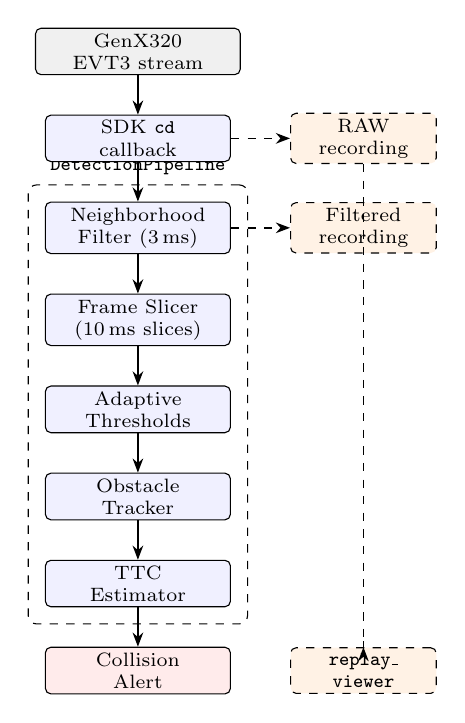
\begin{tikzpicture}[
  node distance=0.5cm,
  box/.style={draw, rounded corners=2pt, align=center, font=\scriptsize,
              minimum width=2.35cm, minimum height=0.58cm, inner sep=2pt,
              fill=blue!6},
  hw/.style={box, fill=gray!12, minimum width=2.6cm},
  io/.style={box, dashed, fill=orange!10, minimum width=1.85cm},
  arr/.style={-{Stealth[length=1.8mm]}, semithick},
  darr/.style={arr, dashed}
]
\node[hw] (sensor) {GenX320\\EVT3 stream};
\node[box, below=of sensor] (callback) {SDK \texttt{cd}\\callback};
\node[box, below=of callback] (filter) {Neighborhood\\Filter ($3$\,ms)};
\node[box, below=of filter] (slicer) {Frame Slicer\\($10$\,ms slices)};
\node[box, below=of slicer] (calib) {Adaptive\\Thresholds};
\node[box, below=of calib] (tracker) {Obstacle\\Tracker};
\node[box, below=of tracker] (ttc) {TTC\\Estimator};
\node[box, below=of ttc, fill=red!8] (alert) {Collision\\Alert};

\node[io, right=0.75cm of callback] (raw) {RAW\\recording};
\node[io, right=0.75cm of filter] (filt) {Filtered\\recording};
\node[io, right=0.75cm of alert] (replay) {\texttt{replay\_}\\\texttt{viewer}};

\draw[arr] (sensor) -- (callback);
\draw[arr] (callback) -- (filter);
\draw[arr] (filter) -- (slicer);
\draw[arr] (slicer) -- (calib);
\draw[arr] (calib) -- (tracker);
\draw[arr] (tracker) -- (ttc);
\draw[arr] (ttc) -- (alert);

\draw[darr] (callback.east) -- (raw.west);
\draw[darr] (filter.east) -- (filt.west);
\draw[darr] (raw.south) |- (replay.north);

\begin{scope}[on background layer]
  \node[draw, dashed, rounded corners=3pt, inner sep=6pt,
        fit=(filter)(slicer)(calib)(tracker)(ttc),
        label={[font=\scriptsize]above:\texttt{DetectionPipeline}}] {};
\end{scope}
\end{tikzpicture}%
}
\caption{End-to-end processing pipeline from GenX320 event ingestion to collision alerting. Solid arrows denote the main data path; dashed boxes indicate auxiliary recording and offline replay. All algorithmic stages enclosed in the dashed region are orchestrated by \texttt{DetectionPipeline}.}
\label{fig:pipeline}
\end{figure}

\begin{enumerate}
    \item \textbf{System bootstrap.} The live application (\texttt{optical\_avoidance}) opens the first available Prophesee device via \texttt{Metavision::Camera::from\_first\_available()}, verifies the $320 \times 320$ sensor geometry, and applies hardware bias registers (\texttt{bias\_diff\_on}, \texttt{bias\_diff\_off}) through the low-level \texttt{I\_LL\_Biases} interface to suppress thermal leakage while preserving edge sensitivity. Output directories are created and a \texttt{DetectionPipeline} instance is constructed for the sensor resolution.

    \item \textbf{Asynchronous event ingestion.} Upon \texttt{camera.start()}, the Metavision SDK invokes a registered change-detection (\texttt{cd}) callback whenever a new EVT3 packet arrives. Each callback delivers a contiguous array of raw \texttt{EventCD} tuples $(x, y, p, t)$ without blocking the sensor driver. In parallel, the application optionally records the untouched EVT3 stream to disk for later replay.

    \item \textbf{Spatiotemporal neighborhood filtering.} The \texttt{NeighborhoodFilter} appends all incoming events to a temporal deque and discards entries older than $3\text{ ms}$ relative to the newest timestamp. It then rebuilds a $320 \times 320$ occupancy map counting active pixels within that window. Each candidate event survives only if the sum of its four cardinal neighbors (North, South, East, West) on the map is at least $N_{\min} = 1$, eliminating isolated hot pixels and uncorrelated background noise \cite{b15}. Surviving events are written both to the next pipeline stage and to a filtered binary recording file.

    \item \textbf{Temporal slicing.} The \texttt{FrameSlicer} accumulates filtered events and partitions them into non-overlapping $10\text{ ms}$ windows anchored to the first observed timestamp. Whenever an event timestamp crosses a slice boundary, the slicer emits a completed \texttt{TimeSlice} containing all events from that interval and resets its buffer. At shutdown, any residual events are flushed as a final partial slice.

    \item \textbf{Adaptive background calibration.} During the first $30$ emitted slices, the \texttt{AdaptiveThresholds} module records the per-slice event count without triggering detections. After calibration, it computes the median count and derives two dynamic thresholds: a slice-level detection threshold ($\max(35,\; 2 \times \text{median})$) and a sector-level minimum ($\max(10,\; \lfloor\text{median}/2\rfloor + 5)$). These thresholds adapt the pipeline to ambient activity levels without manual tuning.

    \item \textbf{Sector-wise geometric tracking.} For each completed slice, the \texttt{ObstacleTracker} first rejects slices whose event count falls below the adaptive detection threshold (further moderated by a $12\%$ relative floor). Remaining events are partitioned into three vertical sectors---Left ($x \leq 106$), Central ($107 \leq x \leq 213$), and Right ($x \geq 214$)---and per-sector statistics (min/max coordinates, event count, coordinate sums) are accumulated in a single pass. The sector with the highest event count becomes dominant; its axis-aligned bounding box and arithmetic centroid are computed. If the dominant sector count is below the sector threshold (with an $8\%$ relative floor), the slice is classified as clear. Otherwise, the inter-slice centroid displacement yields a discrete motion direction (left, right, up, down, or stationary) when the displacement exceeds $3$ pixels.

    \item \textbf{Kinematic TTC estimation.} The \texttt{TtcEstimator} maintains an independent $60\text{ ms}$ area history per sector. For each valid track, the current bounding-box area $A(t)$ is appended to the history of the dominant sector. Net area growth $\Delta A$ over the oldest sample in the window is divided by the elapsed time $\Delta t$ to obtain a growth rate $\dot{A} = \Delta A / \Delta t$ (in px$^2$/s). A collision-relevant expansion is confirmed only when $\dot{A} \geq 1500$ and the relative growth $\Delta A / A_{\text{base}} \geq 25\%$, which rejects periodic on-site motion (e.g., rotating blades) that oscillates around a stable baseline. When expansion is confirmed, $\text{TTC} = A(t) / \dot{A}$ is computed in seconds and smoothed via exponential moving average ($\alpha = 0.4$). If expansion ceases, the TTC estimate decays by a factor of $0.6$ per slice until invalidated.

    \item \textbf{Collision decision and alerting.} A danger flag is raised when the smoothed TTC of the actively expanding sector drops below $\tau_{\text{danger}} = 0.45\text{ s}$. The decision engine formats a sector-specific alert string (e.g., \textit{KOLIZJA CENTRALNY TTC=0.32 s}) and exposes it to the console output layer. When no valid track is present, previously stored TTC values decay gracefully rather than persisting stale warnings.

    \item \textbf{Output and graceful shutdown.} Each processed slice updates a single-line console status showing centroid coordinates, bounding-box dimensions, motion direction, dominant sector, and active event count; danger states append a visual warning marker. On \texttt{SIGINT}/\texttt{SIGTERM}, raw and filtered recordings are flushed and closed, the camera is stopped, and any buffered slices are processed through the same pipeline via \texttt{flush()}.
\end{enumerate}

The offline \texttt{replay\_viewer} replays steps 3--8 identically by feeding recorded EVT3 files through the same \texttt{DetectionPipeline}, rendering each slice as a green-on-black event frame with sector dividers, bounding boxes, centroids, and TTC overlays for visual inspection.

\subsection{Computational Performance and Latency Evaluation}
The main objective of the performance benchmarks was to measure the execution latency per event packet and verify whether the pipeline could continuously process high-rate event streams on the Raspberry Pi 5 without introducing data desynchronization or dropping critical packets.

\begin{table}[htbp]
\caption{Measured Per-Stage Processing Latency on Raspberry Pi 5 ($\Delta T = 10\text{ ms}$; GenX320 recording of $7.14$\,M events at $320\times320$). The filter is timed per SDK packet; the tracker and TTC estimator per $10\text{ ms}$ slice.}
\begin{center}
\begin{tabular}{|l|c|c|c|}
\hline
\textbf{Pipeline Stage} & \textbf{Mean [$\mu$s]} & \textbf{p99 [$\mu$s]} & \textbf{Max [$\mu$s]} \\
\hline
Neighborhood Filter (packet) & 11.7 & 34.3 & 1618 \\
Geometric Tracker (slice)    & 14.2 & 97.1 & 838 \\
TTC Estimator (slice)        & 0.9  & 20.1 & 91 \\
\hline
\textbf{Tracker + TTC (slice)} & \textbf{15.1} & \textbf{104.5} & \textbf{839} \\
\hline
\end{tabular}
\label{tab:latency}
\end{center}
\end{table}

\begin{table}[htbp]
\caption{Aggregate Throughput and Resource Metrics Over the Full Recording}
\begin{center}
\begin{tabular}{|l|c|}
\hline
\textbf{Metric} & \textbf{Value} \\
\hline
Events processed              & $7.14$\,M \\
Event-time span               & $26.6$\,s \\
Total CPU processing time     & $350$\,ms \\
Throughput                    & $20.4$\,Mev/s \\
Real-time factor              & $76\times$ \\
Mean core cost per $10$\,ms slice & $0.13$\,ms ($1.3\%$ of budget) \\
Slices exceeding $10$\,ms budget  & $0\%$ \\
Filter event rejection        & $27.6\%$ \\
Peak filter buffer / TTC history  & $9830$\,ev / $7$\,samples \\
\hline
\end{tabular}
\label{tab:aggregate}
\end{center}
\end{table}

As shown in Table~\ref{tab:latency}, the most expensive per-slice stage is the geometric tracker at a mean of $14.2\ \mu\text{s}$, while the TTC estimator is effectively negligible ($0.9\ \mu\text{s}$). The spatiotemporal filter, timed per SDK packet, averages $11.7\ \mu\text{s}$; since roughly ten packets feed each $10\text{ ms}$ slice, the filter aggregates to the single largest contributor to per-slice cost. Critically, this cost is dominated by the fixed maintenance of the $320 \times 320$ occupancy map (an $O(W \times H)$ rebuild per packet) rather than by the event count. Aggregated over the full recording (Table~\ref{tab:aggregate}), the pipeline consumes only $350\text{ ms}$ of CPU time to process $26.6\text{ s}$ of event data---a $76\times$ real-time margin. The mean core cost per $10\text{ ms}$ accumulation window is approximately $0.13\text{ ms}$, i.e. under $1.3\%$ of the real-time budget, and no slice exceeded the $10\text{ ms}$ deadline (the p99 of the tracker+TTC stage is $104.5\ \mu\text{s}$). This ultra-low execution footprint leaves the remaining CPU cores fully available to handle high-level UAV autopilot flight controls and navigation routines.

The geometric reduction loops ($\min$, $\max$, and $\sum$ over event coordinates) are auto-vectorized by GCC under \texttt{-O3 -mcpu=cortex-a76}, exploiting ARM NEON SIMD lanes to evaluate multiple coordinates per clock cycle. Empirically, the tracker scales linearly with the number of events $N$ per slice at $\approx 9\text{ ns}$ per event, confirming the theoretical $O(N)$ complexity of the single-pass reduction. Profiling further reveals that the principal fixed cost of the pipeline is not event-proportional but stems from clearing and rebuilding the filter's $320 \times 320$ occupancy map once per packet---an $O(W \times H)$ operation independent of $N$---identifying it as the primary candidate for future optimization (e.g. a timestamp-stamped map that avoids full clears).

\subsection{Comparative Analysis Against Alternative Solutions}
To contextualize the efficiency of our heuristic approach, comparative benchmarks were performed against the traditional frameworks discussed in the literature review. Each framework was tested on the same Raspberry Pi 5 hardware using identical raw event recordings from the GenX320 sensor.

\begin{itemize}
    \item \textbf{Contrast Maximization (CM) \cite{b6}:} Uptime was cut short due to massive computational stalls. The iterative warping of millions of coordinates to evaluate full-frame image variance saturated a single CPU core entirely ($100\%$ core utilization). The execution latency per packet escalated to over $110\text{ ms}$, violating the $10\text{ ms}$ real-time boundary. This caused buffer overflows, data bus throttling, and critical EVT3 stream desynchronization manifested by catastrophic \textit{NonMonotonicTimeHigh} driver errors.
    \item \textbf{Deep Neural Networks (Ev-TTA / ResNet34) \cite{b11}:} Attempting to pass accumulated event frames into a standard ResNet34 model on the Raspberry Pi 5 CPU resulted in an average inference time of $315\text{ ms}$ per frame. This heavy computational demand completely disqualifies deep neural networks for real-time edge-based obstacle avoidance without high-power desktop hardware or dedicated external accelerators.
    \item \textbf{Proposed Bio-Inspired Pipeline:} By replacing heavy global optimization loops and dense networks with localized filtering and bounding-box kinematics \cite{b13}, our system sustained a steady $100\text{ Hz}$ processing cadence with $0\%$ packet loss. On the benchmark recording, the measured single-core CPU load remained consistently below $2\%$ (equivalent to a $76\times$ real-time margin), with per-slice processing under $0.15\text{ ms}$, guaranteeing absolute system stability and real-time collision response with substantial headroom for denser scenes.
\end{itemize}
%%%%%%%%%%%%%%%%%%%%%%%%%%%%%%%%%%%%%%%%%%%%%%%%%%%%%%%%%%%%%%%%%%%%%%%%%%%%%%%%%%%%%%
\section{Conclusion and Future Work}

In this paper, we presented a real-time, ultra-low-latency bio-inspired optical avoidance pipeline deployed on a resource-constrained edge computing platform. By shifting away from computationally intensive paradigms such as Contrast Maximization \cite{b6}, deep neural networks \cite{b5, b11}, and continuous-time SLAM \cite{b10}, we successfully avoided the pitfalls of CPU saturation, data bus throttling, and EVT3 stream desynchronization on the Raspberry Pi 5. The implemented framework leverages a highly efficient 4-way spatiotemporal neighborhood filter for noise suppression \cite{b15}, vectorized ARM NEON SIMD loops for instantaneous 2D Bounding Box extraction \cite{b14}, and a kinematic Time-to-Collision (TTC) estimation metric based on optical footprint expansion \cite{b13}. 

Experimental results confirm that the entire pipeline executes with a mean core latency of approximately 0.13~ms per 10~ms accumulation window, utilizing under 1.3\% of the real-time processing budget while maintaining 0\% packet loss and a $76\times$ real-time margin (350~ms of CPU time for 26.6~s of event data). This minimal overhead proves that reactive, insect-inspired looming detection \cite{b13} can successfully provide autonomous agents with rapid collision alerts without relying on heavy desktop hardware or external accelerators.

Future work will focus on three primary avenues to expand the capabilities and robustness of the current architecture:
\begin{enumerate}
    \item \textbf{Inertial Sensor Fusion:} Integrating continuous-time data from an Inertial Measurement Unit (IMU) \cite{b10}. Aligning high-rate gyroscope and accelerometer streams with the asynchronous event data will allow the system to mathematically compensate for the drone's own ego-motion \cite{b4}. This will prevent false-positive expansion triggers caused by aggressive flight maneuvers or camera rotations.
    \item \textbf{Multi-Obstacle Clustering:} Upgrading the current geometric tracker to handle complex environments containing multiple independent hazards. By replacing the single bounding box abstraction with lightweight, SIMD-optimized clustering techniques (e.g., connected-component labeling adapted for sparse matrices), the system will track and calculate independent TTC vectors for multiple obstacles simultaneously across different spatial sectors.
    \item \textbf{Closed-Loop Flight Integration:} Deploying the application onto an active quadcopter platform to validate physical avoidance maneuvers. The C++ decision engine will be interfaced with an open-source flight controller stack (such as PX4 or ArduPilot) via the MAVLink protocol, translating critical sector-based collision alerts into automated, real-time kinetic evasion vectors.
\end{enumerate}

%%%%%%%%%%%%%%%%%%%%%%%%%%%%%%%%%%%%%%%%%%%%%%%%%%%%%%%%%%%%%%%%%%%%%%%%%%%%%%%%%%%%%%

\section*{Acknowledgment}
The authors would like to thank the Embedded Vision Systems Group for their support and resources during the development of this prototype.
%%%%%%%%%%%%%%%%%%%%%%%%%%%%%%%%%%%%%%%%%%%%%%%
\begin{thebibliography}{00}

\bibitem{b3} G. Gallego et al., ``Event-based Vision: A Survey,'' IEEE Trans. Pattern Anal. Mach. Intell., vol. 44, no. 1, pp. 154--180, Jan. 2022.

\bibitem{b5} P. Wzorek and T. Kryjak, ``Traffic Sign Detection With Event Cameras and DCNN,'' in arXiv preprint arXiv:2207.13345, 2022.

\bibitem{b11} J. Kim, I. Hwang, and Y. M. Kim, ``Ev-TTA: Test-Time Adaptation for Event-Based Object Recognition,'' in Proc. IEEE/CVF Conf. Comput. Vis. Pattern Recognit. (CVPR), June 2022, pp. 17745--17754.

\bibitem{b10} E. Mueggler, G. Gallego, H. Rebecq, and D. Scaramuzza, ``Continuous-Time Visual-Inertial Odometry for Event Cameras,'' IEEE Trans. Robot., vol. 34, no. 6, pp. 1425--1440, Dec. 2018.

\bibitem{b6} G. Gallego, H. Rebecq, and D. Scaramuzza, ``A Unifying Contrast Maximization Framework for Event Cameras, with Applications to Motion, Depth, and Optical Flow Estimation,'' IEEE Trans. Pattern Anal. Mach. Intell., vol. 42, no. 10, pp. 2503--2519, Oct. 2019.

\bibitem{b15} J. Wu et al., ``A Spatiotemporal Noise Filtering Algorithm for Event-Based Vision Sensors,'' in Proc. IEEE International Conference on Image Processing (ICIP), 2020, pp. 1103--1107.

\bibitem{b14} T. Delbruck and M. Lang, ``Robotic Goalie with 3 ms Reaction Time at 4\% CPU Load Using Event-Based Dynamic Vision Sensor,'' Frontiers in Neuroscience, vol. 7, p. 223, 2013.

\bibitem{b13} T. Clady et al., ``Asynchronous Visual Event-Based Time-to-Contact,'' Frontiers in Neuroscience, vol. 9, p. 137, 2015.

\bibitem{b4} E. Mueggler, B. Huber, and D. Scaramuzza, ``Event-based, 6-DOF pose tracking for high-speed maneuvers,'' in Proc. IEEE/RSJ Int. Conf. Intell. Robots Syst. (IROS), 2014, pp. 2761--2768.

\bibitem{b12} S. Tulyakov, D. Gehri, et al., ``Time Lens: Event-based Video Frame Interpolation,'' in Proc. IEEE Conf. Comput. Vis. Pattern Recognit. (CVPR), 2021.

\bibitem{b9} S. Zhu, Z. Tang, M. Yang, E. Learned-Miller, and D. Kim, ``Event Camera-based Visual Odometry for Dynamic Motion Tracking of a Legged Robot Using Adaptive Time Surface,'' in Proc. IEEE/RSJ Int. Conf. Intell. Robots Syst. (IROS), Oct. 2023.

\bibitem{b8} C. Scheerlinck, H. Rebecq, T. Stoffregen, N. Barnes, R. Mahony, and D. Scaramuzza, ``CED: Color Event Camera Dataset,'' in Proc. IEEE Winter Conf. Appl. Comput. Vis. (WACV), Mar. 2020, pp. 1391--1400.

\bibitem{b1} K. Chaney, F. Cladera, Z. Wang, A. Bisulco, M. A. Hsieh, C. Korpela, V. Kumar, C. J. Taylor, and K. Daniilidis, ``M3ED: Multi-Robot, Multi-Sensor, Multi-Environment Event Dataset,'' in Proc. IEEE Conf. Comput. Vis. Pattern Recognit. (CVPR), June 2024, pp. 22618--22628.

\bibitem{b2} S. Zhu, Z. Xiong, and D. Kim, ``EAGLE: The First Event Camera Dataset Gathered by an Agile Quadruped Robot,'' arXiv preprint arXiv:2404.04698, 2024.

\bibitem{b7} S. M. Low and D. K. Liu, ``EV-PropNet: Real-time Visual Odometry from Event-based Data,'' in Proc. IEEE Int. Conf. Robot. Autom. (ICRA), May 2017, pp. 2022--2029.

\end{thebibliography}
\end{document}